A global picture of the system interaction with actors is provided here by means of use case diagrams. Following, an analysis of the most interesting use case situations derived from scenarios is presented.

	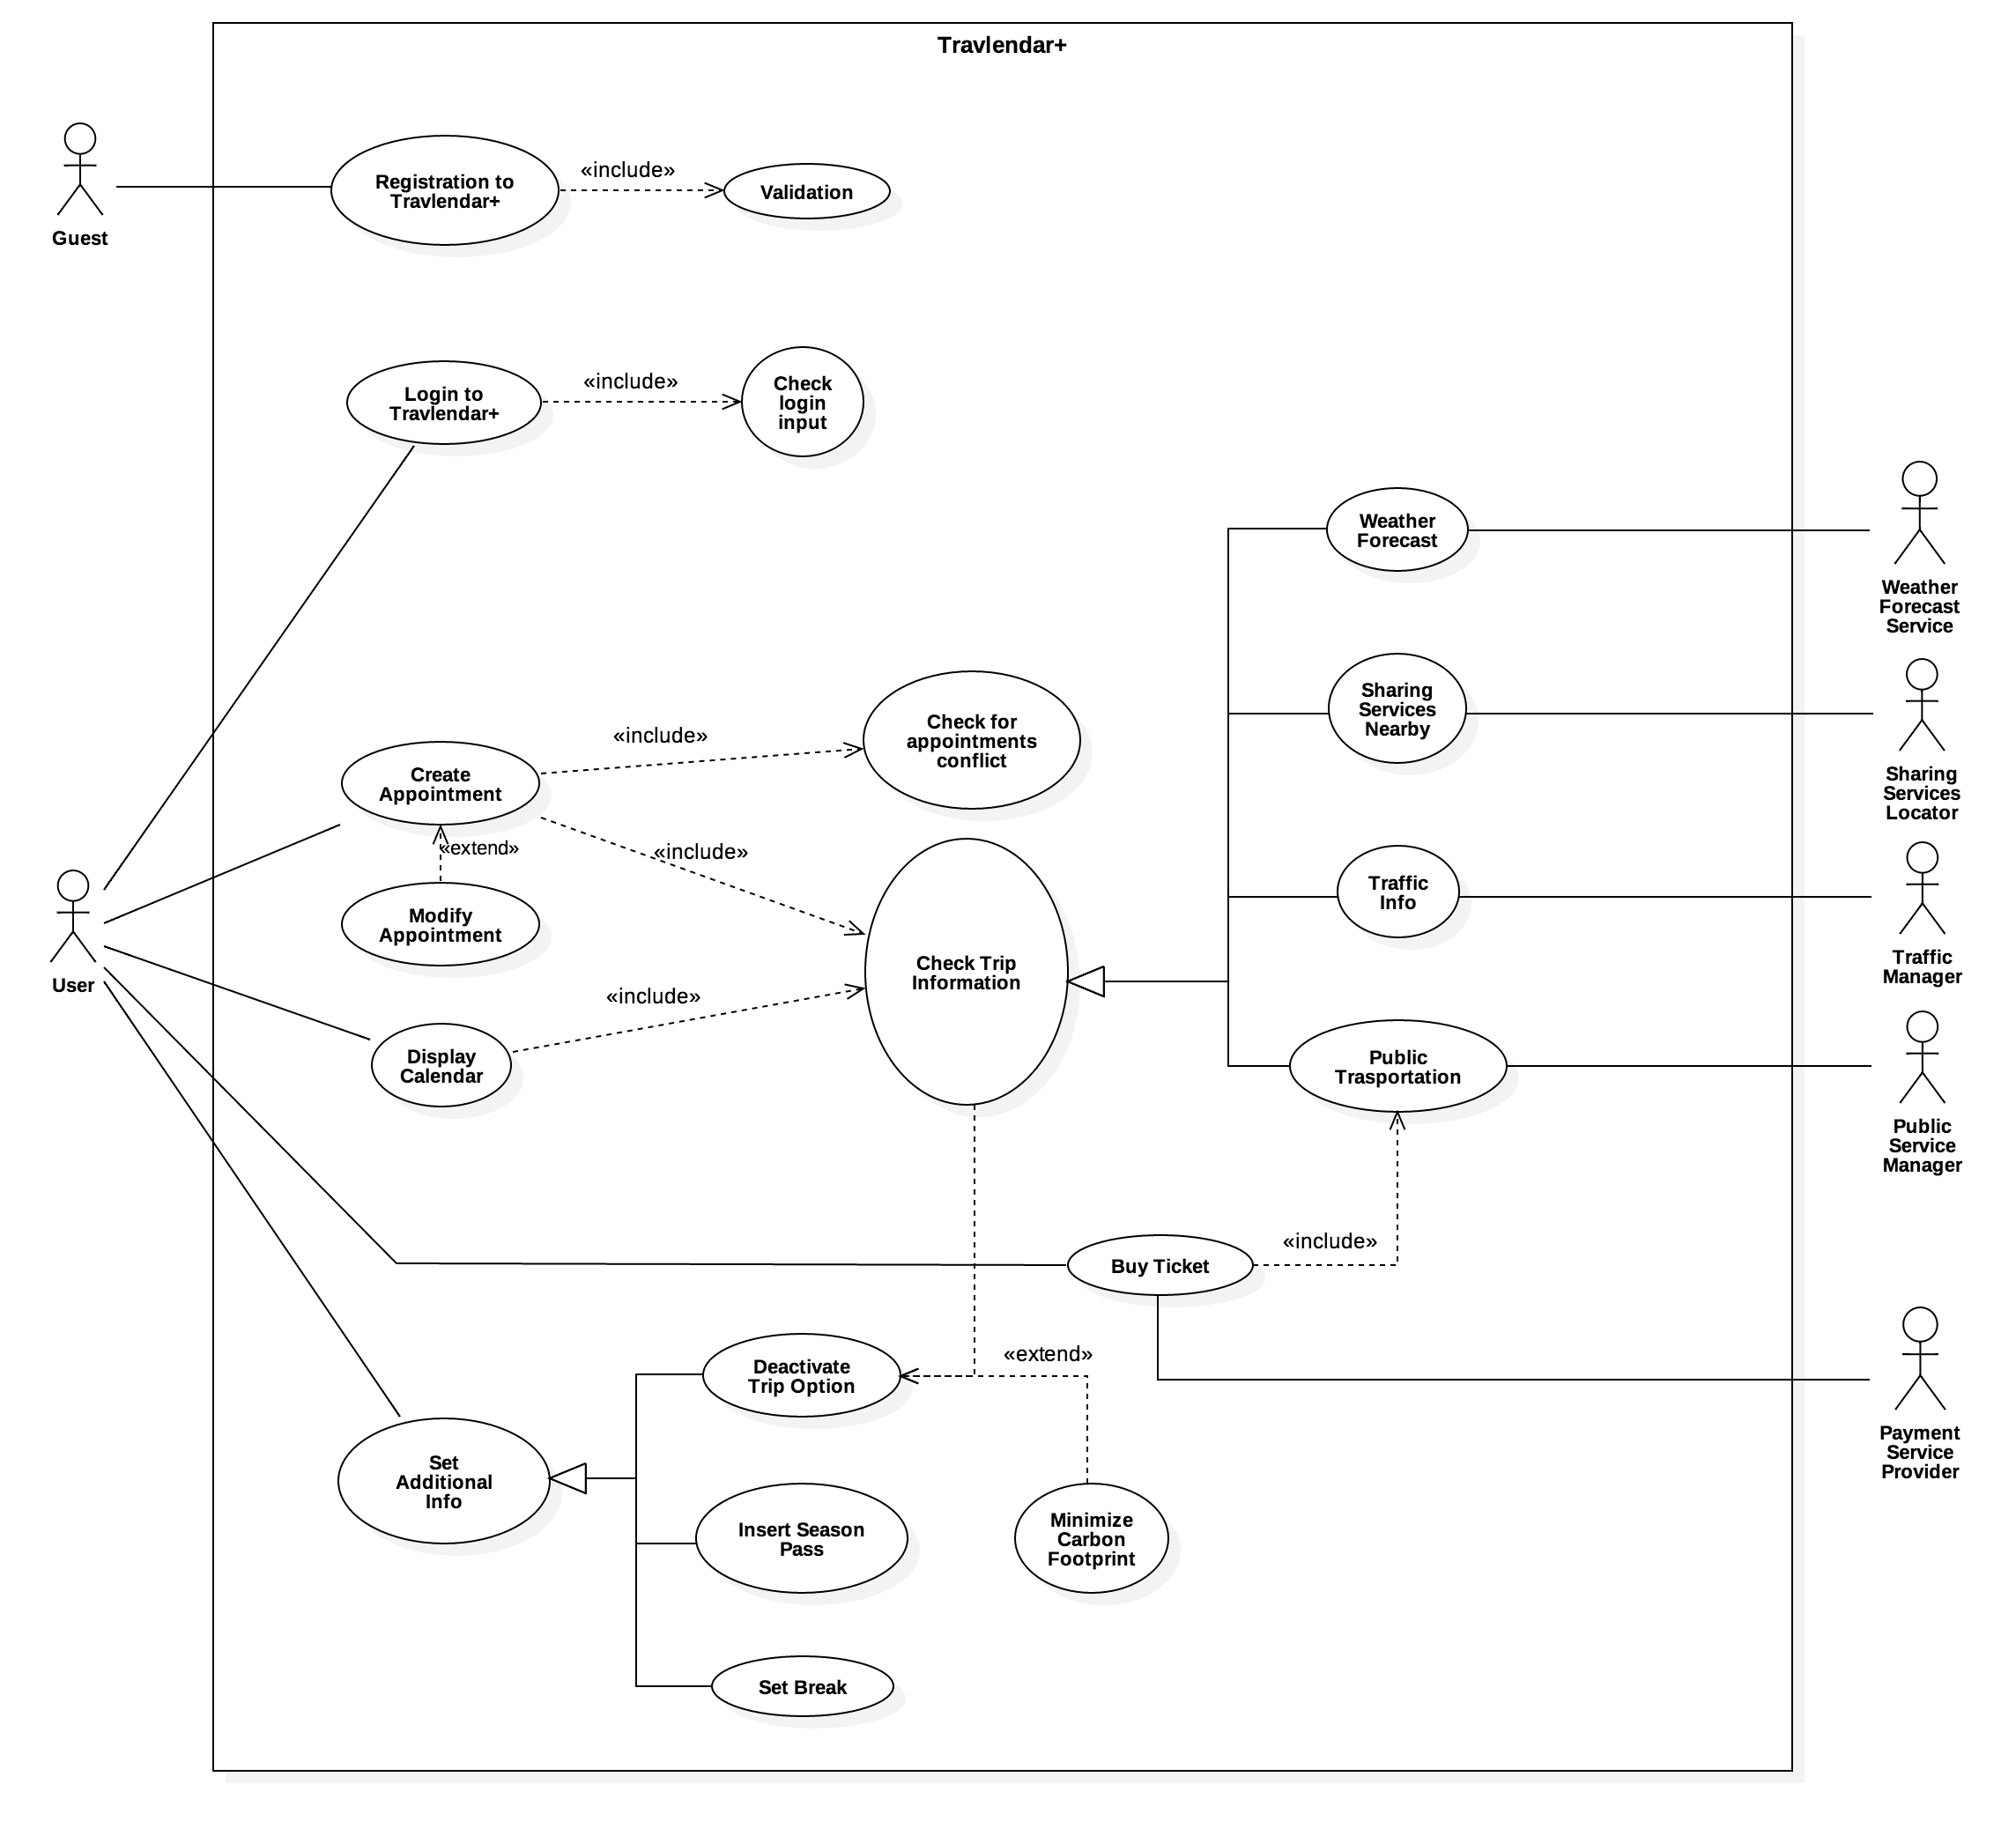
\includegraphics[width=\textwidth]{uml/useCase}


%%% REGISTER %%%	
	\paragraph{Guest registers to \textit{Travlendar+}}\label{login_useCase}
		\begin{table}[H]
			\begin{tabular}{| l | p{0.8\textwidth} | }
				\hline
				\hline
				Actor	&		Guest. \\
				\hline
				Input Condition		&		NULL. \\
				\hline
				Event Flow		&		\begin{enumerate}
													\item Guest clicks on "Sign Up" button.
													\item Guest fills in at least all mandatory fields.
													\item Guest reads and accepts privacy policies and agreements from the company.
													\item Guest clicks on "Confirm" button.
													\item System sends Guest a confirmation link to the provided e-mail.
													\item Guest clicks on the confirmation link.
													\item	 System saves the data in the DB.
												\end{enumerate} \\
				\hline
				Output Condition		&		Guest succesfully ends registration process and become a User. From now on he/she can log in to the application using his/her credential and start using \textit{Tralvendar+}. \\
				\hline		
				Exception		&		\begin{itemize}
												\item[-] Guest is already a User.
												\item[-] One or more mandatory fields are not valid.
												\item[-] Choosen username is already in use.
												\item[-] Email choosen is already associated to another user.
											\end{itemize}
											All exception are handle alerting the visitor of the problem and application goes back to point 2 of Event Flow \\
				\hline
				\hline
			\end{tabular}
			\caption{Guest Register Use Case}
		\end{table}

%%% LOGIN %%%	
	\paragraph{Guest logins into \textit{Travlendar+}}\label{login_useCase}
	
		\begin{table}[H]
			\begin{tabular}{| l | p{0.8\textwidth} | }
				\hline
				\hline
				Actor	&		Guest, User. \\
				\hline
				Input Condition		&		Guest is registered to  \textit{Travlendar+}. \\
				\hline
				Event Flow		&		\begin{enumerate}
													\item Guest fills login mandatory fields.
													\item Guest clicks on "Log In" button.
													\item System verifies login credentials.
												\end{enumerate} \\
				\hline
				Output Condition		&		Guest is promoted to User and is shown is Calendar home page. \\
				\hline		
				Exception		&		Login credentials are incorrect and Guest is shows again Login page\\
				\hline
				\hline
			\end{tabular}
			\caption{Guest Login Use Case}
		\end{table}

%%% CREATE A NEW APPOINTMENT %%%	
	\paragraph{Create a New Appointment} \label{createEvent_useCase}
	
		\begin{table}[H]
			\begin{tabular}{| l | p{0.8\textwidth} | }
				\hline
				\hline
				Actor	&		User. \\
				\hline
				Input Condition		&		User is already logged in into \textit{Travlendar+}. \\
				\hline
				Event Flow		&		\begin{enumerate}
													\item User clicks on "Create Appointment".
													\item User sets name, day, time and position of the Appointment.
													\item System checks if the new appointment overlaps with already existing appointments or break period.
													\item	 System calculates, ranks and shows multiple solutions depending on user travelling preferences.
													\item User selects one of the proposed solutions as preferend one.
												\end{enumerate} \\
				\hline
				Output Condition		&		\textit{Tralvendar+} shows calendar main page with the new appointment. \\
				\hline		
				Exception		&		\begin{itemize}
												\item[-] Created appointment overlaps with already existing appointments.
												\item[-] There are no feasible solution.
												\item[-] Inserted location isn't in the \textit{Operative Zone}.
											\end{itemize} \\
				\hline
				\hline
			\end{tabular}
			\caption{Create new Appointment Use Case}
		\end{table}


%%% MODIFY APPOINTMENT %%%

	\paragraph{Modify appointment}
	
		\begin{table}[H]
			\begin{tabular}{| l | p{0.8\textwidth} | }
				\hline
				\hline
				Actor	&		User. \\
				\hline
				Input Condition		&		\begin{itemize}
														\item[-] User is already logged in into \textit{Travlendar+}.
														\item[-] Appointment already exists.
													\end{itemize} \\
				\hline
				Event Flow		&		\begin{enumerate}
													\item User clicks on "Appointment".
													\item User starts modifying process.
													\item System checks if the new appointment overlap with already existing appointments or break period.
													\item	 System calculates, ranks and shows multiple solution depending on user travelling preferences.
													\item User selects one of the proposed solutions as preferend one.
												\end{enumerate} \\
				\hline
				Output Condition		&		\textit{Tralvendar+} shows calendar main page, with the updated appointment. \\
				\hline		
				Exception		&		\begin{itemize}
												\item[-] Modified appointment overlaps with already existing appointments.
												\item[-] There are no more feasible solutions.
												\item[-] Modified location is no more in the \textit{Operative Zone}.
											\end{itemize} \\
				\hline
				\hline
			\end{tabular}
			\caption{Modify an Appointment Use Case}
		\end{table}
		
%%% INSERT PAYMENT METHOD%%%

	\paragraph{Insert Payment Method}
	
		\begin{table}[H]
			\begin{tabular}{| l | p{0.8\textwidth} | }
				\hline
				\hline
				Actor	&		User. \\
				\hline
				Input Condition		&		\begin{itemize}
														\item[-] User is already logged in into \textit{Travlendar+}.
														\item[-] Credit Card isn't already inserted on the system.
													\end{itemize} \\
				\hline
				Event Flow		&		\begin{enumerate}
													\item User clicks on "Preferences/Payment Methods".
													\item User sets all the credit cards info.
													\item System checks and validate provided informations.
												\end{enumerate} \\
				\hline
				Output Condition		&		\textit{Tralvendar+} returns to "Payment Methods" page showing added card as a valid payment method.\\	
				\hline		
				Exception		&		Credit card given informations are invalid. \\
				\hline
				\hline
			\end{tabular}
			\caption{Insert a Payment Method Use Case}
		\end{table}

%%% BUY TICKET %%%

	\paragraph{Buy Public Transportation Ticket} \label{buyTicket_useCase}
		\begin{table}[H]
			\begin{tabular}{| l | p{0.8\textwidth} | }
				\hline
				\hline
				Actor	&		User. \\
				\hline
				Input Condition		&		\begin{itemize}
														\item[-] User is already in "Solutions" page.
														\item[-] A payment method is already available.
													\end{itemize} \\
				\hline
				Event Flow		&		\begin{enumerate}
													\item User clicks on "desired solution".
													\item User clicks on "Buy Ticket" button.
													\item System shows available public trasportation tickets.
													\item User selects a ticket.
													\item	 System starts purchase transaction.
												\end{enumerate} \\
				\hline
				Output Condition		&		Based on public transportation service, User receives a valid ticket. \\
				\hline		
				Exception		&		\textit{External Transaction Service} doesn't worked as expected. \\
				\hline
				\hline
			\end{tabular}
			\caption{Buy Public Transportation Ticket Use Case}
		\end{table}

%%%  RESERVE SHARING SERVICE %%%

	\paragraph{Reserve a \textit{Sharing Service} Resource} \label{sharing_useCase}
		
		\begin{table}[H]
			\begin{tabular}{| l | p{0.8\textwidth} | }
				\hline
				\hline
				Actor	&		User. \\
				\hline
				Input Condition		&		\begin{itemize}
														\item[-] User is already in "Solutions" page.
														\item[-] A "Sharing mean" is already available.
														\item[-] A "payment method" is already available.
														\item[-] User is in the \textit{influence zone}
													\end{itemize} \\
				\hline
				Event Flow		&		\begin{enumerate}
													\item System connects to available "Sharing Service" resources.
													\item System ranks per distance all the freasible recources and shows them on a map centered on User position.
													\item User chooses one on the possible solutions.												
													\item User clicks on "Reserve it" button.
													\item	 System reconnects to selected \textit{Sharing Service}, and starts the reserving procedure.
												\end{enumerate} \\
				\hline
				Output Condition		&		User redirected to the \textit{Reservation Service} app. \\
				\hline		
				Exception		&		\textit{Reservation Service} doesn't worked as expected. \\
				\hline
				\hline
			\end{tabular}
			\caption{Reserve a Sharing Service Resource Use Case}
		\end{table}
		
%%%  SET TRIP PREFERENCES%%%

	\paragraph{Set Trip Preferences}
	
		\begin{table}[H]
			\begin{tabular}{| l | p{0.8\textwidth} | }
				\hline
				\hline
				Actor	&		User. \\
				\hline
				Input Condition		&		User is already logged in into \textit{Travlendar+}. \\
				\hline
				Event Flow		&		\begin{enumerate}
													\item User click on "Preferences/Trip".
													\item System shows all the possible preferences.
													\item User pins prefered options.
												\end{enumerate} \\
				\hline
				Output Condition		&		\begin{itemize}
														\item[-] User returns to Caledar page.
														\item[-] System recalculate all future trip solution according to User preferences.
														\item[-] User is informed of particular problem
													\end{itemize} \\
				\hline
				Exception		&		User unpins all the possible travel means. \\	
				\hline
				\hline
			\end{tabular}
			\caption{Set Trip Preferences Use Case}
		\end{table}
		
%%%  SET BREAK %%%

	\paragraph{Set Break Period}
		
		\begin{table}[H]
			\begin{tabular}{| l | p{0.8\textwidth} | }
				\hline
				\hline
				Actor	&		User. \\
				\hline
				Input Condition		&		User is already logged in into \textit{Travlendar+}. \\
				\hline
				Event Flow		&		\begin{enumerate}
													\item User clicks on "Preferences/Breaks".
													\item User selects an interval and a minimum lenght for his break.
												\end{enumerate} \\
				\hline
				Output Condition		&		System adds those hours as a special meeting every day in the calendar. \\
				\hline
				\hline
			\end{tabular}
			\caption{Set Break Period}
		\end{table}